\documentclass[conference]{IEEEtran}
\IEEEoverridecommandlockouts
\usepackage{amsmath,amssymb,amsfonts}
\usepackage{graphicx}
\usepackage{booktabs}
\usepackage{multirow}
\usepackage{algorithm}
\usepackage{algpseudocode}
\usepackage{xcolor}
\usepackage{url}
\usepackage[hidelinks]{hyperref}
\makeatletter\setlength{\@fptop}{0pt}\makeatother
\newcommand{\CostScorerShare}{76}
\newcommand{\CreditXGBbase}{0.4338}
\newcommand{\DiscOracleNatsHi}{17}
\newcommand{\DiscOracleNatsLo}{13}
\newcommand{\FidHistErr}{0.010}
\newcommand{\FidHistN}{2{,}000}
\newcommand{\ScorerCalls}{64{,}813}
\newcommand{\SpBatDefault}{4.5}
\newcommand{\SpBatMax}{6.2}
\newcommand{\SpBatMin}{3.9}
\newcommand{\SpBatX}{5.1}
\newcommand{\SpConfigs}{6}
\newcommand{\SpOrigDefault}{22.8}

\newcommand{\CpuFullOverOne}{30}
\newcommand{\CpuSecFive}{21}
\newcommand{\CpuSecFour}{139}
\newcommand{\CpuSecFull}{1{,}017}
\newcommand{\CpuSecOne}{33}
\newcommand{\CpuSecTwo}{56}
\newcommand{\CrConcHi}{2.0}
\newcommand{\CrConcLo}{1.6}
\newcommand{\CrEqPS}{2{,}225}
\newcommand{\CrEqPSCpu}{1.9}
\newcommand{\CrEqPSCpuSec}{64}
\newcommand{\CrEqPSGpu}{1.8}
\newcommand{\CrEqPSGpuSec}{2.6}
\newcommand{\CrEqPSX}{2.2}
\newcommand{\CrEqPlatt}{1{,}292}
\newcommand{\CrEqPlattCpu}{1.2}
\newcommand{\CrEqPlattCpuSec}{40}
\newcommand{\CrEqPlattGpu}{1.2}
\newcommand{\CrEqPlattGpuSec}{1.7}
\newcommand{\CrEqPlattX}{1.3}
\newcommand{\CrEqScan}{2{,}152}
\newcommand{\CrEqScanCpu}{1.8}
\newcommand{\CrEqScanCpuSec}{61}
\newcommand{\CrEqScanGpu}{1.7}
\newcommand{\CrEqScanGpuSec}{2.5}
\newcommand{\CrEqScanX}{2.2}
\newcommand{\CrEqXgb}{4{,}140}
\newcommand{\CrEqXgbCpu}{4.4}
\newcommand{\CrEqXgbCpuSec}{145}
\newcommand{\CrEqXgbGpu}{3.7}
\newcommand{\CrEqXgbGpuSec}{5.3}
\newcommand{\CrEqXgbX}{4.1}
\newcommand{\CrFiveAudit}{33/37}
\newcommand{\CrFiveBeta}{3.9}
\newcommand{\CrFiveBetaHarm}{0}
\newcommand{\CrFiveBetaHi}{6.0}
\newcommand{\CrFiveBetaLo}{1.7}
\newcommand{\CrFiveFrozenLL}{0.452}
\newcommand{\CrFiveInterv}{10/10}
\newcommand{\CrFiveIso}{3.8}
\newcommand{\CrFiveIsoHarm}{1}
\newcommand{\CrFiveIsoHi}{6.9}
\newcommand{\CrFiveIsoLo}{0.7}
\newcommand{\CrFivePS}{9.9}
\newcommand{\CrFivePSHarm}{0}
\newcommand{\CrFivePSHi}{13.9}
\newcommand{\CrFivePSLo}{5.9}
\newcommand{\CrFivePlatt}{3.7}
\newcommand{\CrFivePlattHarm}{0}
\newcommand{\CrFivePlattHi}{5.9}
\newcommand{\CrFivePlattLo}{1.6}
\newcommand{\CrFiveScan}{8.7}
\newcommand{\CrFiveScanHarm}{0}
\newcommand{\CrFiveScanHi}{12.4}
\newcommand{\CrFiveScanLo}{5.0}
\newcommand{\CrFiveTemp}{2.4}
\newcommand{\CrFiveTempHarm}{0}
\newcommand{\CrFiveTempHi}{4.4}
\newcommand{\CrFiveTempLo}{0.4}
\newcommand{\CrFiveXgb}{15.6}
\newcommand{\CrFiveXgbHarm}{0}
\newcommand{\CrFiveXgbHi}{19.1}
\newcommand{\CrFiveXgbLo}{12.1}
\newcommand{\CrFourAudit}{5/7}
\newcommand{\CrFourBeta}{1.6}
\newcommand{\CrFourBetaHarm}{0}
\newcommand{\CrFourBetaHi}{2.3}
\newcommand{\CrFourBetaLo}{0.9}
\newcommand{\CrFourFrozenLL}{0.435}
\newcommand{\CrFourInterv}{6/10}
\newcommand{\CrFourIso}{-1.3}
\newcommand{\CrFourIsoHarm}{4}
\newcommand{\CrFourIsoHi}{2.4}
\newcommand{\CrFourIsoLo}{-5.0}
\newcommand{\CrFourPS}{1.5}
\newcommand{\CrFourPSHarm}{0}
\newcommand{\CrFourPSHi}{2.1}
\newcommand{\CrFourPSLo}{0.9}
\newcommand{\CrFourPlatt}{1.6}
\newcommand{\CrFourPlattHarm}{0}
\newcommand{\CrFourPlattHi}{2.1}
\newcommand{\CrFourPlattLo}{1.0}
\newcommand{\CrFourScan}{0.8}
\newcommand{\CrFourScanHarm}{0}
\newcommand{\CrFourScanHi}{1.5}
\newcommand{\CrFourScanLo}{0.2}
\newcommand{\CrFourTemp}{1.5}
\newcommand{\CrFourTempHarm}{0}
\newcommand{\CrFourTempHi}{2.1}
\newcommand{\CrFourTempLo}{1.0}
\newcommand{\CrFourXgb}{2.9}
\newcommand{\CrFourXgbHarm}{0}
\newcommand{\CrFourXgbHi}{3.9}
\newcommand{\CrFourXgbLo}{1.9}
\newcommand{\CrFull}{15{,}000}
\newcommand{\CrFullAudit}{1/5}
\newcommand{\CrFullBeta}{1.5}
\newcommand{\CrFullBetaHarm}{0}
\newcommand{\CrFullBetaHi}{1.8}
\newcommand{\CrFullBetaLo}{1.2}
\newcommand{\CrFullFrozenLL}{0.430}
\newcommand{\CrFullInterv}{5/10}
\newcommand{\CrFullIso}{-1.2}
\newcommand{\CrFullIsoHarm}{4}
\newcommand{\CrFullIsoHi}{0.8}
\newcommand{\CrFullIsoLo}{-3.2}
\newcommand{\CrFullPS}{1.2}
\newcommand{\CrFullPSHarm}{1}
\newcommand{\CrFullPSHi}{1.6}
\newcommand{\CrFullPSLo}{0.7}
\newcommand{\CrFullPlatt}{1.3}
\newcommand{\CrFullPlattHarm}{0}
\newcommand{\CrFullPlattHi}{1.5}
\newcommand{\CrFullPlattLo}{1.1}
\newcommand{\CrFullScan}{0.3}
\newcommand{\CrFullScanHarm}{1}
\newcommand{\CrFullScanHi}{0.7}
\newcommand{\CrFullScanLo}{-0.1}
\newcommand{\CrFullTemp}{1.5}
\newcommand{\CrFullTempHarm}{0}
\newcommand{\CrFullTempHi}{1.7}
\newcommand{\CrFullTempLo}{1.3}
\newcommand{\CrFullXgb}{1.3}
\newcommand{\CrFullXgbHarm}{0}
\newcommand{\CrFullXgbHi}{1.8}
\newcommand{\CrFullXgbLo}{0.8}
\newcommand{\CrLabCpu}{19}
\newcommand{\CrLabCtx}{11{,}500}
\newcommand{\CrLabGap}{9.3}
\newcommand{\CrLabGpu}{18}
\newcommand{\CrLabLL}{0.4306}
\newcommand{\CrOneAudit}{20/22}
\newcommand{\CrOneBeta}{2.1}
\newcommand{\CrOneBetaHarm}{0}
\newcommand{\CrOneBetaHi}{3.4}
\newcommand{\CrOneBetaLo}{0.9}
\newcommand{\CrOneFrozenLL}{0.444}
\newcommand{\CrOneInterv}{8/10}
\newcommand{\CrOneIso}{1.5}
\newcommand{\CrOneIsoHarm}{4}
\newcommand{\CrOneIsoHi}{3.6}
\newcommand{\CrOneIsoLo}{-0.5}
\newcommand{\CrOnePS}{4.7}
\newcommand{\CrOnePSHarm}{0}
\newcommand{\CrOnePSHi}{7.0}
\newcommand{\CrOnePSLo}{2.3}
\newcommand{\CrOnePlatt}{2.0}
\newcommand{\CrOnePlattHarm}{0}
\newcommand{\CrOnePlattHi}{3.2}
\newcommand{\CrOnePlattLo}{0.8}
\newcommand{\CrOneScan}{4.4}
\newcommand{\CrOneScanHarm}{0}
\newcommand{\CrOneScanHi}{6.9}
\newcommand{\CrOneScanLo}{1.9}
\newcommand{\CrOneTemp}{1.6}
\newcommand{\CrOneTempHarm}{0}
\newcommand{\CrOneTempHi}{2.7}
\newcommand{\CrOneTempLo}{0.5}
\newcommand{\CrOneXgb}{9.0}
\newcommand{\CrOneXgbHarm}{0}
\newcommand{\CrOneXgbHi}{11.6}
\newcommand{\CrOneXgbLo}{6.3}
\newcommand{\CrScanOneLL}{0.4399}
\newcommand{\CrSignHi}{81}
\newcommand{\CrSignLo}{72}
\newcommand{\CrTwoAudit}{10/14}
\newcommand{\CrTwoBeta}{2.2}
\newcommand{\CrTwoBetaHarm}{0}
\newcommand{\CrTwoBetaHi}{3.0}
\newcommand{\CrTwoBetaLo}{1.4}
\newcommand{\CrTwoFrozenLL}{0.440}
\newcommand{\CrTwoInterv}{9/10}
\newcommand{\CrTwoIso}{0.9}
\newcommand{\CrTwoIsoHarm}{1}
\newcommand{\CrTwoIsoHi}{2.1}
\newcommand{\CrTwoIsoLo}{-0.2}
\newcommand{\CrTwoPS}{3.1}
\newcommand{\CrTwoPSHarm}{0}
\newcommand{\CrTwoPSHi}{4.1}
\newcommand{\CrTwoPSLo}{2.0}
\newcommand{\CrTwoPlatt}{2.0}
\newcommand{\CrTwoPlattHarm}{0}
\newcommand{\CrTwoPlattHi}{2.8}
\newcommand{\CrTwoPlattLo}{1.3}
\newcommand{\CrTwoScan}{2.2}
\newcommand{\CrTwoScanHarm}{0}
\newcommand{\CrTwoScanHi}{3.4}
\newcommand{\CrTwoScanLo}{1.0}
\newcommand{\CrTwoTemp}{2.0}
\newcommand{\CrTwoTempHarm}{0}
\newcommand{\CrTwoTempHi}{2.8}
\newcommand{\CrTwoTempLo}{1.3}
\newcommand{\CrTwoXgb}{6.0}
\newcommand{\CrTwoXgbHarm}{0}
\newcommand{\CrTwoXgbHi}{8.0}
\newcommand{\CrTwoXgbLo}{4.0}
\newcommand{\GpuFullOverOne}{27}
\newcommand{\GpuSecFive}{1.0}
\newcommand{\GpuSecFour}{5.1}
\newcommand{\GpuSecFull}{38.9}
\newcommand{\GpuSecOne}{1.4}
\newcommand{\GpuSecTwo}{2.3}
\newcommand{\IclConcHi}{2.4}
\newcommand{\IclConcLo}{2.2}
\newcommand{\IclCpuFullOverOne}{23}
\newcommand{\IclCpuSecFour}{81}
\newcommand{\IclCpuSecFull}{488}
\newcommand{\IclCpuSecOne}{21}
\newcommand{\IclCrEqPS}{1{,}738}
\newcommand{\IclCrEqPSCpu}{1.6}
\newcommand{\IclCrEqPSGpu}{1.0}
\newcommand{\IclCrEqPlatt}{1{,}244}
\newcommand{\IclCrEqPlattCpu}{1.2}
\newcommand{\IclCrEqPlattGpu}{1.0}
\newcommand{\IclCrEqScan}{1{,}371}
\newcommand{\IclCrEqScanCpu}{1.3}
\newcommand{\IclCrEqScanGpu}{1.0}
\newcommand{\IclCrEqXgb}{3{,}860}
\newcommand{\IclCrEqXgbCpu}{3.7}
\newcommand{\IclCrEqXgbGpu}{1.3}
\newcommand{\IclCrOnePS}{4.1}
\newcommand{\IclCrOnePlatt}{2.0}
\newcommand{\IclCrOneScan}{2.9}
\newcommand{\IclCrOneXgb}{8.1}
\newcommand{\IclGpuFullOverOne}{4.7}
\newcommand{\IclGpuSecFour}{2.4}
\newcommand{\IclGpuSecFull}{8.7}
\newcommand{\IclGpuSecOne}{1.8}
\newcommand{\IclPlEqPS}{4{,}060}
\newcommand{\IclPlEqPSCpu}{3.9}
\newcommand{\IclPlEqPSGpu}{1.3}
\newcommand{\IclPlEqPlatt}{1{,}611}
\newcommand{\IclPlEqPlattCpu}{1.5}
\newcommand{\IclPlEqPlattGpu}{1.0}
\newcommand{\IclPlEqScan}{3{,}067}
\newcommand{\IclPlEqScanCpu}{2.9}
\newcommand{\IclPlEqScanGpu}{1.1}
\newcommand{\IclPlEqXgb}{3{,}426}
\newcommand{\IclPlEqXgbCpu}{3.2}
\newcommand{\IclPlEqXgbGpu}{1.1}
\newcommand{\IclPlOnePS}{10.4}
\newcommand{\IclPlOnePlatt}{2.5}
\newcommand{\IclPlOneScan}{9.0}
\newcommand{\IclPlOneXgb}{9.5}
\newcommand{\IclSignHi}{82}
\newcommand{\IclSignLo}{71}
\newcommand{\LadFiles}{240}
\newcommand{\LadSeeds}{10}
\newcommand{\NuFiveBeta}{2.0}
\newcommand{\NuFiveBetaHarm}{4}
\newcommand{\NuFiveBetaHi}{4.2}
\newcommand{\NuFiveBetaLo}{-0.2}
\newcommand{\NuFiveFrozenLL}{0.296}
\newcommand{\NuFiveInterv}{10/10}
\newcommand{\NuFiveIso}{-2.7}
\newcommand{\NuFiveIsoHarm}{7}
\newcommand{\NuFiveIsoHi}{0.3}
\newcommand{\NuFiveIsoLo}{-5.8}
\newcommand{\NuFivePS}{4.1}
\newcommand{\NuFivePSHarm}{0}
\newcommand{\NuFivePSHi}{5.7}
\newcommand{\NuFivePSLo}{2.5}
\newcommand{\NuFivePlatt}{2.0}
\newcommand{\NuFivePlattHarm}{2}
\newcommand{\NuFivePlattHi}{4.2}
\newcommand{\NuFivePlattLo}{-0.1}
\newcommand{\NuFiveScan}{4.1}
\newcommand{\NuFiveScanHarm}{0}
\newcommand{\NuFiveScanHi}{5.9}
\newcommand{\NuFiveScanLo}{2.4}
\newcommand{\NuFiveTemp}{1.2}
\newcommand{\NuFiveTempHarm}{2}
\newcommand{\NuFiveTempHi}{2.9}
\newcommand{\NuFiveTempLo}{-0.5}
\newcommand{\NuFiveXgb}{8.8}
\newcommand{\NuFiveXgbHarm}{0}
\newcommand{\NuFiveXgbHi}{12.4}
\newcommand{\NuFiveXgbLo}{5.2}
\newcommand{\NuFourBeta}{1.6}
\newcommand{\NuFourBetaHarm}{2}
\newcommand{\NuFourBetaHi}{2.8}
\newcommand{\NuFourBetaLo}{0.3}
\newcommand{\NuFourFrozenLL}{0.284}
\newcommand{\NuFourInterv}{7/10}
\newcommand{\NuFourIso}{-3.4}
\newcommand{\NuFourIsoHarm}{6}
\newcommand{\NuFourIsoHi}{1.9}
\newcommand{\NuFourIsoLo}{-8.8}
\newcommand{\NuFourPS}{1.6}
\newcommand{\NuFourPSHarm}{2}
\newcommand{\NuFourPSHi}{3.0}
\newcommand{\NuFourPSLo}{0.2}
\newcommand{\NuFourPlatt}{1.6}
\newcommand{\NuFourPlattHarm}{2}
\newcommand{\NuFourPlattHi}{2.9}
\newcommand{\NuFourPlattLo}{0.2}
\newcommand{\NuFourScan}{-0.0}
\newcommand{\NuFourScanHarm}{3}
\newcommand{\NuFourScanHi}{1.5}
\newcommand{\NuFourScanLo}{-1.5}
\newcommand{\NuFourTemp}{1.6}
\newcommand{\NuFourTempHarm}{2}
\newcommand{\NuFourTempHi}{2.9}
\newcommand{\NuFourTempLo}{0.3}
\newcommand{\NuFourXgb}{1.1}
\newcommand{\NuFourXgbHarm}{3}
\newcommand{\NuFourXgbHi}{2.2}
\newcommand{\NuFourXgbLo}{0.1}
\newcommand{\NuFull}{6{,}000}
\newcommand{\NuFullBeta}{1.2}
\newcommand{\NuFullBetaHarm}{2}
\newcommand{\NuFullBetaHi}{2.3}
\newcommand{\NuFullBetaLo}{0.1}
\newcommand{\NuFullFrozenLL}{0.282}
\newcommand{\NuFullInterv}{6/10}
\newcommand{\NuFullIso}{-3.5}
\newcommand{\NuFullIsoHarm}{8}
\newcommand{\NuFullIsoHi}{0.8}
\newcommand{\NuFullIsoLo}{-7.8}
\newcommand{\NuFullPS}{0.8}
\newcommand{\NuFullPSHarm}{4}
\newcommand{\NuFullPSHi}{2.5}
\newcommand{\NuFullPSLo}{-0.9}
\newcommand{\NuFullPlatt}{1.3}
\newcommand{\NuFullPlattHarm}{2}
\newcommand{\NuFullPlattHi}{2.5}
\newcommand{\NuFullPlattLo}{0.2}
\newcommand{\NuFullScan}{-0.8}
\newcommand{\NuFullScanHarm}{3}
\newcommand{\NuFullScanHi}{0.6}
\newcommand{\NuFullScanLo}{-2.3}
\newcommand{\NuFullTemp}{1.5}
\newcommand{\NuFullTempHarm}{3}
\newcommand{\NuFullTempHi}{2.7}
\newcommand{\NuFullTempLo}{0.3}
\newcommand{\NuFullXgb}{0.5}
\newcommand{\NuFullXgbHarm}{3}
\newcommand{\NuFullXgbHi}{1.3}
\newcommand{\NuFullXgbLo}{-0.3}
\newcommand{\NuHarmHi}{5}
\newcommand{\NuHarmLo}{3}
\newcommand{\NuOneBeta}{1.7}
\newcommand{\NuOneBetaHarm}{4}
\newcommand{\NuOneBetaHi}{3.4}
\newcommand{\NuOneBetaLo}{0.1}
\newcommand{\NuOneFrozenLL}{0.289}
\newcommand{\NuOneInterv}{7/10}
\newcommand{\NuOneIso}{-7.5}
\newcommand{\NuOneIsoHarm}{9}
\newcommand{\NuOneIsoHi}{-2.3}
\newcommand{\NuOneIsoLo}{-12.7}
\newcommand{\NuOnePS}{2.6}
\newcommand{\NuOnePSHarm}{1}
\newcommand{\NuOnePSHi}{4.5}
\newcommand{\NuOnePSLo}{0.7}
\newcommand{\NuOnePlatt}{1.5}
\newcommand{\NuOnePlattHarm}{4}
\newcommand{\NuOnePlattHi}{3.1}
\newcommand{\NuOnePlattLo}{-0.0}
\newcommand{\NuOneScan}{1.9}
\newcommand{\NuOneScanHarm}{1}
\newcommand{\NuOneScanHi}{4.5}
\newcommand{\NuOneScanLo}{-0.7}
\newcommand{\NuOneTemp}{1.3}
\newcommand{\NuOneTempHarm}{3}
\newcommand{\NuOneTempHi}{2.8}
\newcommand{\NuOneTempLo}{-0.2}
\newcommand{\NuOneXgb}{3.8}
\newcommand{\NuOneXgbHarm}{0}
\newcommand{\NuOneXgbHi}{5.8}
\newcommand{\NuOneXgbLo}{1.7}
\newcommand{\NuPSMax}{4.1}
\newcommand{\NuPSMin}{0.8}
\newcommand{\NuTwoBeta}{1.4}
\newcommand{\NuTwoBetaHarm}{3}
\newcommand{\NuTwoBetaHi}{2.9}
\newcommand{\NuTwoBetaLo}{-0.1}
\newcommand{\NuTwoFrozenLL}{0.286}
\newcommand{\NuTwoInterv}{9/10}
\newcommand{\NuTwoIso}{-2.4}
\newcommand{\NuTwoIsoHarm}{8}
\newcommand{\NuTwoIsoHi}{0.5}
\newcommand{\NuTwoIsoLo}{-5.3}
\newcommand{\NuTwoPS}{1.8}
\newcommand{\NuTwoPSHarm}{2}
\newcommand{\NuTwoPSHi}{3.3}
\newcommand{\NuTwoPSLo}{0.4}
\newcommand{\NuTwoPlatt}{1.5}
\newcommand{\NuTwoPlattHarm}{2}
\newcommand{\NuTwoPlattHi}{3.0}
\newcommand{\NuTwoPlattLo}{-0.0}
\newcommand{\NuTwoScan}{0.2}
\newcommand{\NuTwoScanHarm}{5}
\newcommand{\NuTwoScanHi}{2.5}
\newcommand{\NuTwoScanLo}{-2.1}
\newcommand{\NuTwoTemp}{1.2}
\newcommand{\NuTwoTempHarm}{3}
\newcommand{\NuTwoTempHi}{2.5}
\newcommand{\NuTwoTempLo}{-0.1}
\newcommand{\NuTwoXgb}{2.5}
\newcommand{\NuTwoXgbHarm}{0}
\newcommand{\NuTwoXgbHi}{3.7}
\newcommand{\NuTwoXgbLo}{1.3}
\newcommand{\PlConcHi}{4.4}
\newcommand{\PlConcLo}{2.2}
\newcommand{\PlEqPS}{2{,}973}
\newcommand{\PlEqPSCpu}{2.7}
\newcommand{\PlEqPSCpuSec}{90}
\newcommand{\PlEqPSGpu}{2.4}
\newcommand{\PlEqPSGpuSec}{3.4}
\newcommand{\PlEqPSX}{3.0}
\newcommand{\PlEqPlatt}{1{,}238}
\newcommand{\PlEqPlattCpu}{1.2}
\newcommand{\PlEqPlattCpuSec}{39}
\newcommand{\PlEqPlattGpu}{1.2}
\newcommand{\PlEqPlattGpuSec}{1.7}
\newcommand{\PlEqPlattX}{1.2}
\newcommand{\PlEqScan}{4{,}175}
\newcommand{\PlEqScanCpu}{4.4}
\newcommand{\PlEqScanCpuSec}{147}
\newcommand{\PlEqScanGpu}{3.8}
\newcommand{\PlEqScanGpuSec}{5.4}
\newcommand{\PlEqScanX}{4.2}
\newcommand{\PlEqXgb}{3{,}411}
\newcommand{\PlEqXgbCpu}{3.3}
\newcommand{\PlEqXgbCpuSec}{110}
\newcommand{\PlEqXgbGpu}{2.9}
\newcommand{\PlEqXgbGpuSec}{4.1}
\newcommand{\PlEqXgbX}{3.4}
\newcommand{\PlFiveBeta}{3.2}
\newcommand{\PlFiveBetaHarm}{1}
\newcommand{\PlFiveBetaHi}{6.2}
\newcommand{\PlFiveBetaLo}{0.1}
\newcommand{\PlFiveFrozenLL}{0.298}
\newcommand{\PlFiveInterv}{10/10}
\newcommand{\PlFiveIso}{0.3}
\newcommand{\PlFiveIsoHarm}{5}
\newcommand{\PlFiveIsoHi}{4.7}
\newcommand{\PlFiveIsoLo}{-4.0}
\newcommand{\PlFiveJac}{0.48}
\newcommand{\PlFiveOracle}{16.7}
\newcommand{\PlFivePS}{13.1}
\newcommand{\PlFivePSHarm}{0}
\newcommand{\PlFivePSHi}{20.5}
\newcommand{\PlFivePSLo}{5.7}
\newcommand{\PlFivePlatt}{3.1}
\newcommand{\PlFivePlattHarm}{0}
\newcommand{\PlFivePlattHi}{6.2}
\newcommand{\PlFivePlattLo}{0.1}
\newcommand{\PlFiveResFrozen}{0.229}
\newcommand{\PlFiveResPlatt}{0.220}
\newcommand{\PlFiveResScan}{0.143}
\newcommand{\PlFiveScan}{11.5}
\newcommand{\PlFiveScanHarm}{2}
\newcommand{\PlFiveScanHi}{18.2}
\newcommand{\PlFiveScanLo}{4.8}
\newcommand{\PlFiveTemp}{2.2}
\newcommand{\PlFiveTempHarm}{2}
\newcommand{\PlFiveTempHi}{5.4}
\newcommand{\PlFiveTempLo}{-0.9}
\newcommand{\PlFiveXgb}{15.2}
\newcommand{\PlFiveXgbHarm}{0}
\newcommand{\PlFiveXgbHi}{21.4}
\newcommand{\PlFiveXgbLo}{9.1}
\newcommand{\PlFourBeta}{1.9}
\newcommand{\PlFourBetaHarm}{3}
\newcommand{\PlFourBetaHi}{3.8}
\newcommand{\PlFourBetaLo}{-0.0}
\newcommand{\PlFourFrozenLL}{0.278}
\newcommand{\PlFourInterv}{8/10}
\newcommand{\PlFourIso}{-2.9}
\newcommand{\PlFourIsoHarm}{6}
\newcommand{\PlFourIsoHi}{2.0}
\newcommand{\PlFourIsoLo}{-7.9}
\newcommand{\PlFourJac}{0.36}
\newcommand{\PlFourOracle}{9.1}
\newcommand{\PlFourPS}{4.5}
\newcommand{\PlFourPSHarm}{1}
\newcommand{\PlFourPSHi}{8.3}
\newcommand{\PlFourPSLo}{0.8}
\newcommand{\PlFourPlatt}{1.9}
\newcommand{\PlFourPlattHarm}{3}
\newcommand{\PlFourPlattHi}{3.9}
\newcommand{\PlFourPlattLo}{-0.0}
\newcommand{\PlFourResFrozen}{0.172}
\newcommand{\PlFourResPlatt}{0.148}
\newcommand{\PlFourResScan}{0.112}
\newcommand{\PlFourScan}{4.1}
\newcommand{\PlFourScanHarm}{2}
\newcommand{\PlFourScanHi}{8.2}
\newcommand{\PlFourScanLo}{-0.0}
\newcommand{\PlFourTemp}{1.5}
\newcommand{\PlFourTempHarm}{1}
\newcommand{\PlFourTempHi}{2.9}
\newcommand{\PlFourTempLo}{0.1}
\newcommand{\PlFourXgb}{1.9}
\newcommand{\PlFourXgbHarm}{2}
\newcommand{\PlFourXgbHi}{3.7}
\newcommand{\PlFourXgbLo}{-0.0}
\newcommand{\PlFull}{6{,}000}
\newcommand{\PlFullBeta}{1.5}
\newcommand{\PlFullBetaHarm}{3}
\newcommand{\PlFullBetaHi}{2.9}
\newcommand{\PlFullBetaLo}{0.0}
\newcommand{\PlFullFrozenLL}{0.274}
\newcommand{\PlFullInterv}{8/10}
\newcommand{\PlFullIso}{-2.0}
\newcommand{\PlFullIsoHarm}{6}
\newcommand{\PlFullIsoHi}{2.9}
\newcommand{\PlFullIsoLo}{-6.9}
\newcommand{\PlFullJac}{0.31}
\newcommand{\PlFullOracle}{6.8}
\newcommand{\PlFullPS}{3.2}
\newcommand{\PlFullPSHarm}{1}
\newcommand{\PlFullPSHi}{5.6}
\newcommand{\PlFullPSLo}{0.9}
\newcommand{\PlFullPlatt}{1.6}
\newcommand{\PlFullPlattHarm}{3}
\newcommand{\PlFullPlattHi}{3.0}
\newcommand{\PlFullPlattLo}{0.1}
\newcommand{\PlFullResFrozen}{0.148}
\newcommand{\PlFullResPlatt}{0.121}
\newcommand{\PlFullResScan}{0.100}
\newcommand{\PlFullScan}{2.7}
\newcommand{\PlFullScanHarm}{3}
\newcommand{\PlFullScanHi}{6.6}
\newcommand{\PlFullScanLo}{-1.1}
\newcommand{\PlFullTemp}{1.2}
\newcommand{\PlFullTempHarm}{2}
\newcommand{\PlFullTempHi}{2.2}
\newcommand{\PlFullTempLo}{0.1}
\newcommand{\PlFullXgb}{1.1}
\newcommand{\PlFullXgbHarm}{2}
\newcommand{\PlFullXgbHi}{1.8}
\newcommand{\PlFullXgbLo}{0.4}
\newcommand{\PlLabCpu}{6}
\newcommand{\PlLabCtx}{5{,}200}
\newcommand{\PlLabGap}{2.1}
\newcommand{\PlLabGpu}{5}
\newcommand{\PlLabLL}{0.2755}
\newcommand{\PlOneBeta}{1.5}
\newcommand{\PlOneBetaHarm}{3}
\newcommand{\PlOneBetaHi}{3.0}
\newcommand{\PlOneBetaLo}{0.1}
\newcommand{\PlOneFrozenLL}{0.289}
\newcommand{\PlOneInterv}{10/10}
\newcommand{\PlOneIso}{-2.2}
\newcommand{\PlOneIsoHarm}{7}
\newcommand{\PlOneIsoHi}{0.7}
\newcommand{\PlOneIsoLo}{-5.1}
\newcommand{\PlOneJac}{0.56}
\newcommand{\PlOneOracle}{16.0}
\newcommand{\PlOnePS}{8.6}
\newcommand{\PlOnePSHarm}{1}
\newcommand{\PlOnePSHi}{14.6}
\newcommand{\PlOnePSLo}{2.6}
\newcommand{\PlOnePlatt}{1.5}
\newcommand{\PlOnePlattHarm}{2}
\newcommand{\PlOnePlattHi}{2.8}
\newcommand{\PlOnePlattLo}{0.1}
\newcommand{\PlOneResFrozen}{0.226}
\newcommand{\PlOneResPlatt}{0.214}
\newcommand{\PlOneResScan}{0.113}
\newcommand{\PlOneScan}{11.6}
\newcommand{\PlOneScanHarm}{0}
\newcommand{\PlOneScanHi}{16.9}
\newcommand{\PlOneScanLo}{6.3}
\newcommand{\PlOneTemp}{0.9}
\newcommand{\PlOneTempHarm}{2}
\newcommand{\PlOneTempHi}{1.9}
\newcommand{\PlOneTempLo}{-0.1}
\newcommand{\PlOneXgb}{9.8}
\newcommand{\PlOneXgbHarm}{0}
\newcommand{\PlOneXgbHi}{13.2}
\newcommand{\PlOneXgbLo}{6.4}
\newcommand{\PlOracleShareHi}{73}
\newcommand{\PlOracleShareLo}{69}
\newcommand{\PlScanOneLL}{0.2776}
\newcommand{\PlSignHi}{77}
\newcommand{\PlSignLo}{76}
\newcommand{\PlTwoBeta}{1.9}
\newcommand{\PlTwoBetaHarm}{3}
\newcommand{\PlTwoBetaHi}{4.2}
\newcommand{\PlTwoBetaLo}{-0.4}
\newcommand{\PlTwoFrozenLL}{0.284}
\newcommand{\PlTwoInterv}{10/10}
\newcommand{\PlTwoIso}{-4.7}
\newcommand{\PlTwoIsoHarm}{7}
\newcommand{\PlTwoIsoHi}{1.8}
\newcommand{\PlTwoIsoLo}{-11.3}
\newcommand{\PlTwoJac}{0.56}
\newcommand{\PlTwoOracle}{14.1}
\newcommand{\PlTwoPS}{6.5}
\newcommand{\PlTwoPSHarm}{3}
\newcommand{\PlTwoPSHi}{12.2}
\newcommand{\PlTwoPSLo}{0.9}
\newcommand{\PlTwoPlatt}{1.9}
\newcommand{\PlTwoPlattHarm}{3}
\newcommand{\PlTwoPlattHi}{4.0}
\newcommand{\PlTwoPlattLo}{-0.2}
\newcommand{\PlTwoResFrozen}{0.212}
\newcommand{\PlTwoResPlatt}{0.194}
\newcommand{\PlTwoResScan}{0.104}
\newcommand{\PlTwoScan}{8.7}
\newcommand{\PlTwoScanHarm}{4}
\newcommand{\PlTwoScanHi}{16.0}
\newcommand{\PlTwoScanLo}{1.4}
\newcommand{\PlTwoTemp}{1.2}
\newcommand{\PlTwoTempHarm}{3}
\newcommand{\PlTwoTempHi}{2.4}
\newcommand{\PlTwoTempLo}{0.0}
\newcommand{\PlTwoXgb}{5.4}
\newcommand{\PlTwoXgbHarm}{1}
\newcommand{\PlTwoXgbHi}{8.6}
\newcommand{\PlTwoXgbLo}{2.3}
\newcommand{\PlattSignHi}{52}
\newcommand{\PlattSignLo}{40}
\newcommand{\ScanRulesCrOne}{2.2}
\newcommand{\ScanSecMax}{16}
\newcommand{\ScanSecMed}{5.5}
\newcommand{\ScanSecOneMed}{7.0}
\newcommand{\XgbLeavesCr}{418}

\newcommand{\BBiasHi}{0.16}
\newcommand{\BBiasLo}{0.15}
\newcommand{\BCalRedHi}{22}
\newcommand{\BCalRedLo}{1}
\newcommand{\BCatCrAUC}{0.777}
\newcommand{\BCatCrBeta}{0.2}
\newcommand{\BCatCrIso}{-1.8}
\newcommand{\BCatCrLL}{0.4332}
\newcommand{\BCatCrPS}{0.3}
\newcommand{\BCatCrPlatt}{0.2}
\newcommand{\BCatCrRep}{1/10}
\newcommand{\BCatCrScan}{0.1}
\newcommand{\BCatNuAUC}{0.730}
\newcommand{\BCatNuBeta}{-0.4}
\newcommand{\BCatNuIso}{-4.3}
\newcommand{\BCatNuLL}{0.2845}
\newcommand{\BCatNuPS}{-0.5}
\newcommand{\BCatNuPlatt}{-0.3}
\newcommand{\BCatNuRep}{2/10}
\newcommand{\BCatNuScan}{-0.5}
\newcommand{\BCatPlAUC}{0.764}
\newcommand{\BCatPlBeta}{0.9}
\newcommand{\BCatPlIso}{-1.9}
\newcommand{\BCatPlLL}{0.2750}
\newcommand{\BCatPlPS}{1.5}
\newcommand{\BCatPlPlatt}{0.9}
\newcommand{\BCatPlRep}{3/10}
\newcommand{\BCatPlScan}{0.7}
\newcommand{\BIclCrAUC}{0.785}
\newcommand{\BIclCrBeta}{1.3}
\newcommand{\BIclCrIso}{-1.8}
\newcommand{\BIclCrLL}{0.4298}
\newcommand{\BIclCrPS}{1.4}
\newcommand{\BIclCrPlatt}{1.4}
\newcommand{\BIclCrRep}{4/10}
\newcommand{\BIclCrScan}{0.3}
\newcommand{\BIclNuAUC}{0.741}
\newcommand{\BIclNuBeta}{1.0}
\newcommand{\BIclNuIso}{-3.6}
\newcommand{\BIclNuLL}{0.2820}
\newcommand{\BIclNuPS}{1.0}
\newcommand{\BIclNuPlatt}{1.1}
\newcommand{\BIclNuRep}{4/10}
\newcommand{\BIclNuScan}{0.1}
\newcommand{\BIclPlAUC}{0.764}
\newcommand{\BIclPlBeta}{1.4}
\newcommand{\BIclPlIso}{-3.4}
\newcommand{\BIclPlLL}{0.2751}
\newcommand{\BIclPlPS}{2.0}
\newcommand{\BIclPlPlatt}{1.4}
\newcommand{\BIclPlRep}{6/10}
\newcommand{\BIclPlScan}{0.9}
\newcommand{\BOracleHi}{7.0}
\newcommand{\BOracleLo}{5.5}
\newcommand{\BPfnCrAUC}{0.784}
\newcommand{\BPfnCrBeta}{1.5}
\newcommand{\BPfnCrIso}{-1.2}
\newcommand{\BPfnCrLL}{0.4297}
\newcommand{\BPfnCrPS}{1.2}
\newcommand{\BPfnCrPlatt}{1.3}
\newcommand{\BPfnCrRep}{5/10}
\newcommand{\BPfnCrScan}{0.3}
\newcommand{\BPfnNuAUC}{0.741}
\newcommand{\BPfnNuBeta}{1.2}
\newcommand{\BPfnNuIso}{-3.5}
\newcommand{\BPfnNuLL}{0.2825}
\newcommand{\BPfnNuPS}{0.8}
\newcommand{\BPfnNuPlatt}{1.3}
\newcommand{\BPfnNuRep}{6/10}
\newcommand{\BPfnNuScan}{-0.8}
\newcommand{\BPfnPlAUC}{0.767}
\newcommand{\BPfnPlBeta}{1.5}
\newcommand{\BPfnPlIso}{-2.0}
\newcommand{\BPfnPlLL}{0.2742}
\newcommand{\BPfnPlPS}{3.2}
\newcommand{\BPfnPlPlatt}{1.6}
\newcommand{\BPfnPlRep}{8/10}
\newcommand{\BPfnPlScan}{2.7}
\newcommand{\BXgbCrAUC}{0.778}
\newcommand{\BXgbCrBeta}{-0.0}
\newcommand{\BXgbCrIso}{-1.8}
\newcommand{\BXgbCrLL}{0.4319}
\newcommand{\BXgbCrPS}{-0.0}
\newcommand{\BXgbCrPlatt}{-0.1}
\newcommand{\BXgbCrRep}{2/10}
\newcommand{\BXgbCrScan}{0.1}
\newcommand{\BXgbNuAUC}{0.732}
\newcommand{\BXgbNuBeta}{-0.2}
\newcommand{\BXgbNuIso}{-5.5}
\newcommand{\BXgbNuLL}{0.2840}
\newcommand{\BXgbNuPS}{-0.3}
\newcommand{\BXgbNuPlatt}{-0.1}
\newcommand{\BXgbNuRep}{3/10}
\newcommand{\BXgbNuScan}{-0.5}
\newcommand{\BXgbPlAUC}{0.752}
\newcommand{\BXgbPlBeta}{0.2}
\newcommand{\BXgbPlIso}{-8.0}
\newcommand{\BXgbPlLL}{0.2780}
\newcommand{\BXgbPlPS}{0.9}
\newcommand{\BXgbPlPlatt}{-0.0}
\newcommand{\BXgbPlRep}{0/10}
\newcommand{\BXgbPlScan}{0.0}
\newcommand{\DBiasCalHi}{0.14}
\newcommand{\DBiasCalLo}{0.11}
\newcommand{\DBiasFHi}{0.15}
\newcommand{\DBiasFLo}{0.13}
\newcommand{\DBiasRedHi}{73}
\newcommand{\DBiasRedLo}{67}
\newcommand{\DBiasSHi}{0.051}
\newcommand{\DBiasSLo}{0.036}
\newcommand{\DCatFourBiasF}{0.134}
\newcommand{\DCatFourBiasP}{0.115}
\newcommand{\DCatFourBiasS}{0.036}
\newcommand{\DCatFourGain}{3.2}
\newcommand{\DCatFourJac}{0.68}
\newcommand{\DCatFourNullHarm}{2}
\newcommand{\DCatFourOracle}{4.7}
\newcommand{\DCatFourRep}{9/10}
\newcommand{\DCatFourShare}{68}
\newcommand{\DCatOneBiasF}{0.134}
\newcommand{\DCatOneBiasP}{0.110}
\newcommand{\DCatOneBiasS}{0.118}
\newcommand{\DCatOneGain}{0.7}
\newcommand{\DCatOneJac}{0.10}
\newcommand{\DCatOneNullHarm}{3}
\newcommand{\DCatOneOracle}{4.8}
\newcommand{\DCatOneRep}{4/10}
\newcommand{\DCatOneShare}{15}
\newcommand{\DIclFourBiasF}{0.153}
\newcommand{\DIclFourBiasP}{0.138}
\newcommand{\DIclFourBiasS}{0.051}
\newcommand{\DIclFourGain}{5.3}
\newcommand{\DIclFourJac}{0.68}
\newcommand{\DIclFourNullHarm}{2}
\newcommand{\DIclFourOracle}{7.0}
\newcommand{\DIclFourRep}{10/10}
\newcommand{\DIclFourShare}{76}
\newcommand{\DIclOneBiasF}{0.153}
\newcommand{\DIclOneBiasP}{0.134}
\newcommand{\DIclOneBiasS}{0.133}
\newcommand{\DIclOneGain}{0.6}
\newcommand{\DIclOneJac}{0.11}
\newcommand{\DIclOneNullHarm}{3}
\newcommand{\DIclOneOracle}{7.0}
\newcommand{\DIclOneRep}{5/10}
\newcommand{\DIclOneShare}{9}
\newcommand{\DJacHi}{0.77}
\newcommand{\DJacLo}{0.68}
\newcommand{\DNullAbsMax}{0.5}
\newcommand{\DNullHarmMax}{2}
\newcommand{\DPfnFourBiasF}{0.154}
\newcommand{\DPfnFourBiasP}{0.129}
\newcommand{\DPfnFourBiasS}{0.049}
\newcommand{\DPfnFourGain}{5.7}
\newcommand{\DPfnFourJac}{0.70}
\newcommand{\DPfnFourNullHarm}{2}
\newcommand{\DPfnFourOracle}{6.9}
\newcommand{\DPfnFourRep}{10/10}
\newcommand{\DPfnFourShare}{84}
\newcommand{\DPfnOneBiasF}{0.154}
\newcommand{\DPfnOneBiasP}{0.125}
\newcommand{\DPfnOneBiasS}{0.116}
\newcommand{\DPfnOneGain}{2.0}
\newcommand{\DPfnOneJac}{0.20}
\newcommand{\DPfnOneNullHarm}{2}
\newcommand{\DPfnOneOracle}{6.9}
\newcommand{\DPfnOneRep}{8/10}
\newcommand{\DPfnOneShare}{28}
\newcommand{\DRepLo}{9}
\newcommand{\DRepOneHi}{8}
\newcommand{\DRepOneLo}{3}
\newcommand{\DShareHi}{84}
\newcommand{\DShareLo}{68}
\newcommand{\DXgbFourBiasF}{0.141}
\newcommand{\DXgbFourBiasP}{0.138}
\newcommand{\DXgbFourBiasS}{0.044}
\newcommand{\DXgbFourGain}{4.2}
\newcommand{\DXgbFourJac}{0.77}
\newcommand{\DXgbFourNullHarm}{0}
\newcommand{\DXgbFourOracle}{5.3}
\newcommand{\DXgbFourRep}{10/10}
\newcommand{\DXgbFourShare}{78}
\newcommand{\DXgbOneBiasF}{0.141}
\newcommand{\DXgbOneBiasP}{0.134}
\newcommand{\DXgbOneBiasS}{0.127}
\newcommand{\DXgbOneGain}{-0.0}
\newcommand{\DXgbOneJac}{0.10}
\newcommand{\DXgbOneNullHarm}{4}
\newcommand{\DXgbOneOracle}{5.4}
\newcommand{\DXgbOneRep}{3/10}
\newcommand{\DXgbOneShare}{-1}
\newcommand{\HistWorse}{12}
\newcommand{\XgbBoostLeaves}{93}


\begin{document}

\title{Fix What the Model Leaves Behind:\\Fast Subgroup Repair for Tree Ensembles\\and Tabular Foundation Models}

% AccML submissions are NOT anonymised: replace with real names and affiliations.
\author{\IEEEauthorblockN{Author Name(s)}
\IEEEauthorblockA{Affiliation(s)\\
email@institution}}

\maketitle

\begin{abstract}
Tabular risk models are deployed as they are: a gradient-boosted ensemble after tuning, or a
tabular foundation model that predicts from labelled rows in its context. Either can be accurate
on average yet systematically wrong for a subgroup defined by a combination of features.
Structured Scan Repair is a post-hoc layer that searches interpretable multi-feature subgroups for
large exact Bernoulli-likelihood gains from a common log-odds shift, validates proposed corrections
on held-out data, and applies a few readable shifts or abstains; the base model itself is never
changed. Across four strong frozen base models (tuned XGBoost and CatBoost, TabPFN-2.5 and
TabICLv2), a planted subgroup error survives base-model construction and global recalibration.
Given enough data to search, the repair removes \DBiasRedLo--\DBiasRedHi\% of it and recovers
\DShareLo--\DShareHi\% of the best possible one-rule gain for every model, without significant
average harm when no subgroup effect is planted. Foundation models add a second lever: more
context, paid for on every prediction. On a context ladder from 500 rows to the full training set,
the repair at 1{,}000 rows matches TabPFN-2.5 at \CrEqScan{} rows on Credit Default and
\PlEqScan{} rows on the planted subgroup, making each prediction \CrEqScanCpu--\PlEqScanCpu$\times$
cheaper on a CPU than the matching context. It preferentially flags observations that benefit from
additional context and moves their predictions in the same direction. The advantage is in recurring
compute: with unlimited compute, placing the held-out labels in the context is more accurate. Compiled, batched scoring makes a fit take seconds on one CPU
core with bit-identical repairs.
\end{abstract}

\begin{IEEEkeywords}
post-hoc model repair, subset scanning, calibration, gradient boosting, tabular foundation models,
in-context learning, inference cost, CPU inference
\end{IEEEkeywords}

%=====================================================================
\section{Introduction}
%=====================================================================
Credit scoring, readmission and churn are standard supervised tabular prediction problems.
Gradient-boosted trees such as XGBoost and CatBoost~\cite{chen2016xgboost,prokhorenkova2018catboost}
remain strong conventional approaches~\cite{grinsztajn2022tree}. Tabular foundation models such as
TabPFN~\cite{hollmann2023tabpfn,hollmann2025nature,grinsztajn2025tabpfn25} and
TabICL~\cite{qu2025tabicl,qu2026tabiclv2} instead use pretrained transformers to predict new rows
from labelled examples supplied in context, without updating their pretrained weights; they are now
competitive with tuned trees~\cite{erickson2025tabarena}. Although the two paradigms construct
predictions differently, once configured both expose the same downstream object: a probability or
logit for each observation. This creates a common interface for asking whether residual predictive
errors can be corrected without modifying the underlying predictor.

A model can be well calibrated on average and still be systematically wrong for a subgroup defined
by a \emph{combination} of features, an error that optimization of average loss need not remove.
Global recalibration (temperature scaling~\cite{guo2017calibration}, Platt~\cite{platt1999},
beta~\cite{kull2017beta}, isotonic regression~\cite{zadrozny2002}, histogram
binning~\cite{zadrozny2001}) applies one common transformation to all predictions and therefore
cannot selectively correct one subgroup without changing predictions elsewhere. Multicalibration,
multiaccuracy and flexible residual learners~\cite{hebert2018multicalibration,kim2019multiaccuracy,tax2026mcgrad}
can correct richer residual structure, but they do not impose the same design goal of returning a
small set of interpretable subgroup shifts that are independently validated and explicitly rejected
when evidence is insufficient. Slice finders~\cite{chung2019slicefinder,sagadeeva2021sliceline}
locate high-loss subsets without repairing them, while predictive-bias scanning~\cite{zhang2016bias},
built on subset scanning~\cite{neill2012fast}, stops at detection. Structured Scan Repair closes
this audit-to-action gap: it searches original features for compact subgroup rules, estimates the
exact likelihood benefit of a log-odds correction, validates that correction independently, and
applies it only if the evidence survives.

We ask two research questions.
\begin{itemize}
\item \textbf{RQ1} (Sec.~\ref{sec:general}). \emph{Does structured repair work across strong
tabular model families?} Tuned XGBoost and CatBoost, TabPFN-2.5 and TabICLv2 all leave the planted
localized error. With sufficient discovery data, Structured Scan removes most of it across all four
backbones without significant average harm when no subgroup effect is planted. In the controlled
planted setting, apparent failures at smaller discovery samples arise from insufficient evidence to
recover the subgroup rather than from absence of the residual.
\item \textbf{RQ2} (Sec.~\ref{sec:ladder}). \emph{For an in-context model, when can repair
substitute for more context?} On a ladder of nested contexts, the repair at 1{,}000 rows matches
TabPFN-2.5 at \CrEqScan--\PlEqScan{} rows, \CrEqScanCpu--\PlEqScanCpu$\times$ cheaper per
prediction on a CPU, and preferentially targets observations that additional context later improves.
As the context grows and the repair opportunity shrinks, it steps aside.
\end{itemize}
The trade in RQ2 needs a repair that is cheap and exact: compiled, batched and parallel candidate
scoring speeds the search \SpBatMin--\SpBatMax$\times$ with bit-identical repairs
(Sec.~\ref{sec:systems}).
%=====================================================================
\section{Structured Scan Repair}\label{sec:method}
%=====================================================================
\textbf{Setting.} A frozen probabilistic classifier outputs a logit $F(x)$ and probability
$p(x)=\sigma(F(x))$. Once repair begins, the base model is never updated: only additive subgroup
shifts are learned. Labelled observations not used to construct the base predictor are partitioned
into \emph{discovery}, \emph{selection} and \emph{test} sets. A subgroup $S$ is an interpretable
conjunction of literals on the original features (numeric thresholds or categorical subsets). After
$T$ accepted corrections, the repaired predictor is
\begin{equation}\label{eq:repair}
F_R(x) = F(x) + \textstyle\sum_{t=1}^{T} \delta_t\, \mathbf{1}[x\in S_t].
\end{equation}

\textbf{Score.} For a candidate subgroup $S$, Structured Scan asks how much the Bernoulli
log-likelihood would improve if every member of $S$ received the same log-odds shift $\delta$:
\begin{equation}\label{eq:gain}
\Delta(S,\delta) = \sum_{i\in S}\Big[y_i\delta - \log\big(1-p_i+e^{\delta}p_i\big)\Big].
\end{equation}
The objective is concave in $\delta$, so Newton iteration gives
$\Delta^\star(S)=\max_\delta\Delta(S,\delta)$. At the optimum,
$\sum_{i\in S}[y_i-\sigma(F_i+\delta)]=0$, so the mean repaired probability within $S$ matches
its observed event rate. The statistic is inherited from predictive-bias scanning~\cite{zhang2016bias};
here it is used not only to detect a biased subgroup but to estimate its correction.

\textbf{Search.} Exhaustively enumerating multi-feature conjunctions is infeasible, so rules grow
one literal at a time in a diversity-aware beam (width 24, maximum depth 5). For a numeric feature
under a parent rule, candidate thresholds are first ranked by the second-order proxy
$\tfrac12 G^2/H$, where $G$ and $H$ are prefix sums of $p_i-y_i$ and $p_i(1-p_i)$ over the sorted
feature. Only a shortlist is evaluated using the exact likelihood gain in~\eqref{eq:gain}.
Categorical levels are ordered so that only prefix subsets need be considered.

\textbf{Validation and abstention.} Discovery proposes candidate rules; selection determines
whether any is sufficiently stable to apply. Each candidate is independently refitted on two
stratified halves $V_1,V_2$ of the selection set. Candidates are retained only when they improve
likelihood on both halves and the fitted shifts have the same sign. Among these, the scanner selects
the rule maximizing the smaller per-row gain across the two halves. A nominal one-degree-of-freedom
likelihood-ratio test for $\delta=0$ is then applied to this single rule on the complete selection
set at $\alpha=0.05$. If it fails, the round terminates; the algorithm does not fall back to a
runner-up. On real data, accepted rules are additionally audited on the test set: subgroup residual
must shrink, removing the rule must worsen test log-loss, and the rule must beat the 95th percentile
of 500 score-matched placebo subgroups. This audit is diagnostic and does not alter the fitted
repair.

\textbf{Iterative repair.} Structured Scan performs at most four rounds. After an accepted rule is
added, all accepted shifts are jointly refitted on selection data with $F$ as a fixed offset and an
$\ell_2$ coefficient penalty of $10^{-3}$. The updated residuals are then scanned again. The process
stops at the first round with no stable candidate or when the selected rule fails the whole-selection
test. Only the subgroup terms in~\eqref{eq:repair} are learned; the parameters, structure and, for
an in-context model, context of the base predictor remain unchanged.

\textbf{Two-stage variant.} Platt$\to$scan fits Platt scaling on discovery data and then applies
Structured Scan to the recalibrated logits; the selection set remains reserved for validating
candidate subgroup corrections. This variant removes a global calibration component before searching
for localized residual structure.

\textbf{What a correction does.} Inside a selected subgroup, adding $\delta$ to the logit
multiplies predicted odds by $e^{\delta}$; observations outside the subgroup are unchanged and
ranking within the subgroup is preserved. Thus a fitted repair is a small collection of explicit
subgroup rules and one scalar shift per rule rather than a second high-capacity predictor.

Algorithm~\ref{alg:ssr} summarizes the fitting procedure. Base-model construction ends before
repair begins; discovery proposes rules, selection decides whether they survive and estimates their
shifts, and test labels are reserved for evaluation and, on real data, the diagnostic audit.

\begin{algorithm}[!t]
\caption{Structured Scan Repair of a frozen classifier}
\label{alg:ssr}
\small
\begin{algorithmic}[1]
\Require Frozen logit $F$; discovery $D$; selection $V=V_1\cup V_2$ (stratified halves);
$T=4$; beam width 24; depth $\leq5$; $\alpha=0.05$; $\ell_2$ penalty $\lambda=10^{-3}$
\Ensure Repaired logit $F_R$ and rule set $\mathcal R$ (possibly empty)
\State $\mathcal R\gets\emptyset$; $F_R\gets F$
\For{$t=1,\ldots,T$}
    \State $\mathcal C\gets$ beam-search rules on $D$, offset $F_R$
    \State for each $S\in\mathcal C$: $(g_h,\hat\delta_h)\gets$ maximize~\eqref{eq:gain} on $V_h$, $h=1,2$
    \State $\mathcal A\gets\{S\in\mathcal C:\ g_1,g_2>0,\ \operatorname{sign}\hat\delta_1=\operatorname{sign}\hat\delta_2\}$
    \If{$\mathcal A=\emptyset$}
        \State \textbf{break} \Comment{abstain from further repair}
    \EndIf
    \State $S_t\gets\arg\max_{S\in\mathcal A}\min_h g_h(S)/|V_h|$ \Comment{most stable}
    \State $p_{\mathrm{LR}}\gets$ nominal 1-df LR $p$-value for $S_t$ on all of $V$
    \If{$p_{\mathrm{LR}}\ge\alpha$}
        \State \textbf{break} \Comment{reject; no runner-up fallback}
    \EndIf
    \State $\mathcal R\gets\mathcal R\cup\{S_t\}$
    \State $\boldsymbol\delta\gets\arg\max\,\ell_V\big(F+\sum_{j\le t}\delta_j\mathbf{1}[x\in S_j]\big)
    -\tfrac{\lambda}{2}\|\boldsymbol\delta\|^2$
    \State $F_R(x)\gets F(x)+\sum_{j\le t}\delta_j\mathbf{1}[x\in S_j]$
\EndFor
\State \Return $F_R,\mathcal R$
\end{algorithmic}
\end{algorithm}
%=====================================================================
\section{Experimental Setup}\label{sec:setup}
%=====================================================================
\textbf{Data and splits.} The controlled synthetic benchmark has $n=12{,}000$ observations and
$p=30$ independent features $X_j\sim\mathrm{Uniform}(0,1)$. A background signal uses the next six
features after the planted-rule variables, with coefficients
$\beta=(1,-0.8,0.7,-0.6,0.5,-0.4)$ applied to centered covariates $2X-1$; the intercept is solved so
that marginal event prevalence is 10\%. The planted subgroup is
$S^*=\{X_1>c,\ldots,X_5>c\}$ with $c=1-0.08^{1/5}\approx0.397$, giving 8\% expected support.
Outcomes follow a Bernoulli logistic model whose logit adds $\log(8)\mathbf{1}[S^*]$ in the planted
condition. The no-planted-effect control uses the same generator with subgroup odds ratio 1: the
six-feature background signal remains, but the additional conjunction effect is absent. Both use
6{,}000 observations for base-model construction and 2{,}400/1{,}800/1{,}800 for
 discovery/selection/test. \emph{Credit Default}~\cite{yeh2009credit} contains 30{,}000 clients and
23 predictors (3 categorical); 15{,}000 observations construct the base model and
6{,}000/4{,}500/4{,}500 form discovery/selection/test. We use ten seeds per setting; within each
seed, every base model and correction uses the same partition. Each synthetic seed is a fresh draw
from the generator; on Credit the 4{,}500 test rows are fixed and the seeds re-partition the
remaining rows.

\textbf{Strong frozen base configurations.} XGBoost and CatBoost are tuned once per dataset by
5-fold cross-validated random search over 25 configurations (log-loss, early stopping) on the first
seed's model-building partition; the selected hyperparameters are then refitted on each seed's
model-building partition and frozen. Tuning never uses test rows. TabPFN-2.5~\cite{grinsztajn2025tabpfn25}
(\texttt{tabpfn} 9.1.0) and TabICLv2~\cite{qu2026tabiclv2} (\texttt{tabicl} 2.2.0) use their
released default configurations and receive the complete model-building split as labelled context.
These protocols provide strong representative configurations rather than exhaustive optimization of
each family. Once base prediction is complete, every model is treated identically by the correction
layer: it receives original features, labels and that model's frozen logits on the common correction
partitions.

\textbf{Preprocessing.} Credit Default has no missing values. Its three categorical variables are
integer-coded using the categories seen in the model-building rows. XGBoost receives these codes as
numeric features; CatBoost, TabPFN-2.5 and TabICLv2 receive them marked as categorical. Scan rules
are reported in the original named feature space. No preprocessing step uses test labels.

\textbf{Post-hoc comparators.} Every correction receives the same correction-data budget; its own
fitting and validation use the common discovery and selection partitions. We evaluate temperature
scaling, Platt scaling, beta calibration, isotonic regression, 15-bin equal-mass histogram binning,
a single residual tree (maximum depth 3, selected on the selection data), a boosted residual
corrector (gradient-boosted trees fitted from the frozen base logit and early-stopped on selection;
median 63--161 leaves per setting), Structured Scan Repair, and Platt$\to$scan. Table~\ref{tab:bench} reports the full cross-model battery; the complete context-ladder table is released with the source.

\textbf{Evaluation and statistical analysis.} The primary metric is test log-loss (LL), reported
absolutely and as improvement over the corresponding frozen base model. For the planted condition
we additionally report absolute residual bias on $S^*$, the \emph{oracle} gain obtained by applying
the optimal one-rule shift to the known subgroup, and Jaccard overlap between the detected and true
subgroups. On Credit we report the held-out audit pass rate; harm counts seeds whose
correction increases test log-loss. Across the ten matched seeds, figures report paired 95\%
confidence intervals where shown, and starred table entries use two-sided paired $t$-tests at
$p<0.05$. These $p$-values are descriptive and are not multiplicity-adjusted.
%=====================================================================
\section{Structured Repair Across Model Families}\label{sec:general}
%=====================================================================
\begin{table*}[t]
\centering
\caption{Frozen-backbone benchmark under the standard correction budget. LL is frozen test log-loss; other entries are mean improvement ($\times10^{-3}$, positive is better) over 10 matched seeds. * paired $p<0.05$ (descriptive, unadjusted); bold: largest mean in the row. Corrections are defined in Sec.~III; P$\to$S: Platt then Scan.}
\label{tab:bench}
\footnotesize\setlength{\tabcolsep}{4pt}
\begin{tabular}{llrrrrrrrrrr}
\toprule
Data & Base model & LL & Temp. & Platt & Beta & Iso. & Hist. & Tree & Boost. & Scan & P$\to$S \\
\midrule
\multirow{4}{*}{Planted} & XGBoost & 0.2780 & +0.0 & $-$0.0 & +0.2 & $-$8.0* & $-$3.0* & $-$0.5 & +0.6* & +0.0 & \textbf{+0.9} \\
 & CatBoost & 0.2750 & +0.1 & +0.9 & +0.9 & $-$1.9 & $-$1.2 & +0.1 & +0.8* & +0.7 & \textbf{+1.5} \\
 & TabPFN-2.5 & 0.2742 & +1.2* & +1.6* & +1.5* & $-$2.0 & $-$2.4* & $-$0.2 & +1.1* & +2.7 & \textbf{+3.2*} \\
 & TabICLv2 & 0.2751 & +1.2* & +1.4* & +1.4* & $-$3.4 & $-$1.7* & $-$0.9 & +0.9* & +0.9 & \textbf{+2.0*} \\
\midrule
\multirow{4}{*}{\begin{tabular}[c]{@{}l@{}}No planted\\effect\end{tabular}} & XGBoost & 0.2840 & $-$0.0 & $-$0.1 & $-$0.2 & $-$5.5* & $-$3.0* & +0.1 & \textbf{+0.3} & $-$0.5 & $-$0.3 \\
 & CatBoost & 0.2845 & $-$0.1 & $-$0.3 & $-$0.4 & $-$4.3 & $-$2.3* & +0.1 & \textbf{+0.4} & $-$0.5 & $-$0.5 \\
 & TabPFN-2.5 & 0.2825 & \textbf{+1.5*} & +1.3* & +1.2* & $-$3.5 & $-$1.1 & $-$0.3 & +0.5 & $-$0.8 & +0.8 \\
 & TabICLv2 & 0.2820 & \textbf{+1.2*} & +1.1 & +1.0* & $-$3.6 & $-$0.8 & +0.1 & +0.2 & +0.1 & +1.0 \\
\midrule
\multirow{4}{*}{Credit} & XGBoost & 0.4319 & $-$0.0 & $-$0.1* & $-$0.0 & $-$1.8* & $-$1.6* & $-$0.2 & \textbf{+0.4*} & +0.1 & $-$0.0 \\
 & CatBoost & 0.4332 & +0.1* & +0.2* & +0.2 & $-$1.8* & $-$1.8* & $-$0.1 & \textbf{+0.4} & +0.1 & +0.3 \\
 & TabPFN-2.5 & 0.4297 & \textbf{+1.5*} & +1.3* & \textbf{+1.5*} & $-$1.2 & $-$1.0* & +0.3 & +1.3* & +0.3 & +1.2* \\
 & TabICLv2 & 0.4298 & \textbf{+1.5*} & +1.4* & +1.3* & $-$1.8 & $-$0.9* & +0.2 & +1.4* & +0.3 & +1.4* \\
\bottomrule
\end{tabular}
\end{table*}


\subsection{Strong predictors leave a common localized residual}
Table~\ref{tab:bench} compares the four frozen base configurations under the standard correction-data
budget. On the planted benchmark their overall test log-loss is similar, yet all four retain
substantial error on the known subgroup: absolute residual bias is \BBiasLo--\BBiasHi, and
correcting the true subgroup with its optimal one-rule shift would improve test log-loss by
\BOracleLo--\BOracleHi$\times10^{-3}$. Global recalibration changes this localized error only
modestly; Platt, beta and isotonic reduce subgroup bias by \BCalRedLo--\BCalRedHi\%. With only 2{,}400 discovery
observations, however, Structured Scan does not recover the subgroup reliably: it accepts a rule in
\BXgbPlRep{} XGBoost, \BCatPlRep{} CatBoost, \BIclPlRep{} TabICLv2 and \BPfnPlRep{} TabPFN-2.5
runs. Consequently, its mean gains at this discovery size are small, whereas Platt$\to$scan gives
the largest mean improvement on the planted condition for all four backbones.

\subsection{Repairability is not the same as detectability}
The weak 2{,}400-row result does not mean that the tree backbones have absorbed the planted
structure. The true subgroup remains worth a similar discovery-set likelihood gain under all four
models (13--17 nats on average). The difficulty is statistical: identifying a five-feature
conjunction among 30 variables from 2{,}400 observations leaves many chance patterns with competitive
scores. We therefore repeat the experiment on a separate $n=19{,}200$ draw and, within that draw,
hold the frozen base models, selection set and test set fixed while varying only the scan's discovery
sample from 2{,}400 to 9{,}600 observations (Table~\ref{tab:disc}, Fig.~\ref{fig:disc}).

With 9{,}600 discovery observations, the earlier backbone dependence largely disappears. Structured
Scan accepts a repair in \DRepLo--10 of 10 runs for every model, recovers
\DShareLo--\DShareHi\% of the best available one-rule gain, and identifies rules with Jaccard
\DJacLo--\DJacHi{} overlap with the true subgroup. The correction reduces absolute subgroup bias
from \DBiasFLo--\DBiasFHi{} to \DBiasSLo--\DBiasSHi, a \DBiasRedLo--\DBiasRedHi\% reduction.
In the matched no-planted-effect control, increasing discovery data does not produce a corresponding
increase in harm: mean Scan gain remains within $\pm$\DNullAbsMax$\times10^{-3}$, with at most
\DNullHarmMax{} harmful seeds. In this controlled setting, the main limitation at the smaller
discovery size is detectability rather than absence of repairable residual structure.

\begin{table}[t]
\centering
\caption{Discovery-power experiment on a separate $n=19{,}200$ draw. Within each model and seed, the frozen predictor, selection set and test set are fixed; Scan receives 2{,}400 or 9{,}600 discovery rows. Gain: mean test log-loss improvement ($\times10^{-3}$); Oracle share: fraction of the best one-rule gain; Jacc.: overlap with the planted subgroup. Null gain (harmful seeds) is from the matched no-planted-effect control.}
\label{tab:disc}
\footnotesize\setlength{\tabcolsep}{2.4pt}
\begin{tabular}{lcrrrcr}
\toprule
Base model & Discovery & \begin{tabular}[b]{@{}c@{}}With\\rule\end{tabular} & Gain & \begin{tabular}[b]{@{}c@{}}Oracle\\share\end{tabular} & Jacc. & \begin{tabular}[b]{@{}c@{}}Null gain\\(harmful seeds)\end{tabular} \\
\midrule
\multirow{2}{*}{XGBoost} & 2.4k & 3/10 & $-$0.0 & 0\% & 0.10 & $-$0.1 (4) \\
 & 9.6k & 10/10 & +4.2* & 78\% & 0.77 & +0.0 (0) \\
\addlinespace[2pt]
\multirow{2}{*}{CatBoost} & 2.4k & 4/10 & +0.7 & 15\% & 0.10 & $-$0.5 (3) \\
 & 9.6k & 9/10 & +3.2* & 68\% & 0.68 & +0.0 (2) \\
\addlinespace[2pt]
\multirow{2}{*}{TabPFN-2.5} & 2.4k & 8/10 & +2.0 & 28\% & 0.20 & +0.2 (2) \\
 & 9.6k & 10/10 & +5.7* & 84\% & 0.70 & +0.5 (2) \\
\addlinespace[2pt]
\multirow{2}{*}{TabICLv2} & 2.4k & 5/10 & +0.6 & 9\% & 0.11 & $-$0.0 (3) \\
 & 9.6k & 10/10 & +5.3* & 76\% & 0.68 & $-$0.1 (2) \\
\bottomrule
\end{tabular}
\end{table}


\begin{figure}[t]
\centering
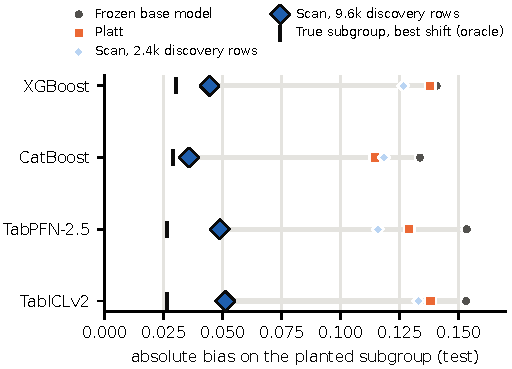
\includegraphics[width=\columnwidth]{fig_disc.pdf}
\caption{Model-agnostic recovery of the planted subgroup in the separate $n=19{,}200$ discovery-power
experiment (test-set absolute residual, mean over 10 seeds; lower is better). Grey circles are frozen
base models; orange squares are Platt; light and dark blue diamonds are Structured Scan with 2{,}400
and 9{,}600 discovery rows; black ticks are the known subgroup with its optimal one-rule shift. The
larger discovery sample moves all four backbones toward the oracle.}
\label{fig:disc}
\end{figure}

\subsection{When little structured residual remains, the scan mostly abstains}
Credit Default presents a different regime. The two foundation models give the strongest frozen
predictions (test LL \BPfnCrLL--\BIclCrLL; AUROC \BPfnCrAUC--\BIclCrAUC), compared with LL
\BXgbCrLL--\BCatCrLL{} for the tuned trees. Across all four backbones, Structured Scan finds little
validated localized residual: it intervenes in only \BCatCrRep--\BPfnCrRep{} runs and changes mean
test log-loss by at most $0.3\times10^{-3}$. The foundation models instead retain modest global
miscalibration, for which Platt and beta improve log-loss by approximately
$1.3$--$1.5\times10^{-3}$; corresponding gains for the tuned trees are at most
$0.2\times10^{-3}$.

The no-planted-effect control shows the same distinction: global recalibration still helps the
foundation models, whereas Scan has near-zero average effect. Across the full correction battery,
isotonic regression and histogram binning tend to overfit, while the boosted residual corrector is
positive in all 12 model--dataset settings and is strongest among the alternatives for several
Credit and control settings. That gain comes from a substantially higher-capacity correction,
typically tens to hundreds of leaves, whereas Structured Scan seeks a small number of named,
held-out-validated subgroup shifts and can return the frozen model unchanged. Thus, when a strong
in-distribution predictor leaves little confirmed localized structure, abstention is part of the
intended behaviour rather than a failed repair.
%=====================================================================
\section{When Should We Repair Rather Than Buy More Context?}\label{sec:ladder}
%=====================================================================
Section~\ref{sec:general} established that the repair is not tied to one model family. We now
narrow to TabPFN-2.5 because context size provides a direct knob for increasing predictive
capability while also increasing recurring inference cost. On a 2-core CPU, TabPFN-2.5 scores
1{,}000 rows in \CpuSecOne\,s from a 1{,}000-row context and in \CpuSecFull\,s from 15{,}000 rows
(\CpuFullOverOne$\times$); a T4 GPU is faster but scales similarly (\GpuSecOne\,s vs.\
\GpuSecFull\,s). We therefore run TabPFN-2.5 on a \emph{ladder} of nested contexts: for each seed,
the model-building split is shuffled once and context $k$ is its first $k$ rows,
$k\in\{500,1\text{k},1.5\text{k},2\text{k},3\text{k},4\text{k},6\text{k},8\text{k},10\text{k}\}$
and full. Logits are saved once per (dataset, seed, $k$); every correction is then fitted on CPU
using the standard correction splits of Sec.~\ref{sec:setup}. This ladder is separate from the
larger discovery-power experiment in Table~\ref{tab:disc}; its numbers should not be chained with
that experiment.

\subsection{Context reduces the repair opportunity}

\begin{figure*}[t]
\centering
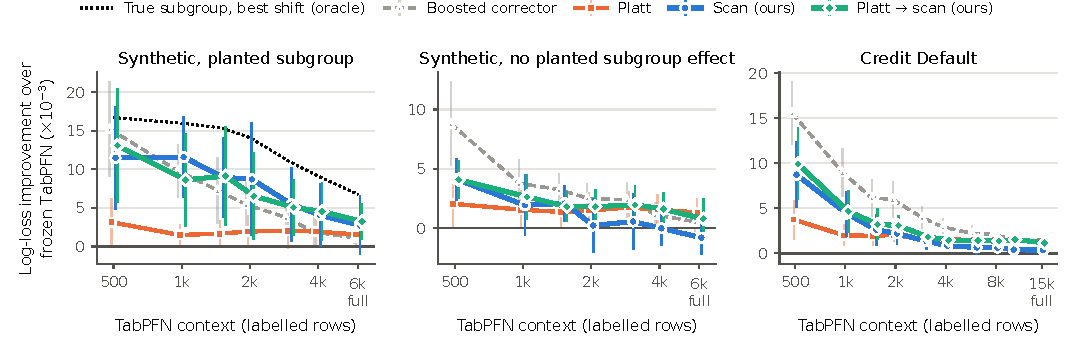
\includegraphics[width=\textwidth]{fig_gain_ladder.pdf}
\caption{Held-out log-loss improvement over frozen TabPFN-2.5 at the same context (mean and paired
95\% CI over 10 seeds; positive is better). The panels show the planted subgroup, the matched
no-planted-effect control, and Credit Default. Global Platt recalibration gives modest gains, whereas
local or flexible corrections can give larger gains at small contexts. Structured Scan contracts as
context grows, tracking the shrinking oracle opportunity in the planted setting.}
\label{fig:gain}
\end{figure*}

Fig.~\ref{fig:gain} shows the main corrections across context; the full correction-by-context table is released with the source. On the planted problem, Structured
Scan improves test log-loss by \PlOneScan$\times10^{-3}$ $[\PlOneScanLo,\PlOneScanHi]$ at 1{,}000
context rows, compared with \PlOnePlatt{} for Platt, and captures
\PlOracleShareLo--\PlOracleShareHi\% of the oracle one-rule gain at 500--1{,}000 rows. From 1{,}000
rows onward it matches or exceeds the boosted residual corrector on this structured error. On Credit,
Scan gains \CrFiveScan{} at 500 rows and \CrOneScan{} $[\CrOneScanLo,\CrOneScanHi]$ at 1{,}000 rows,
although the boosted residual corrector gives the largest raw log-loss improvement throughout the
ladder.

The decline in Scan gain at larger contexts reflects a shrinking target rather than simply poorer
search. On the planted benchmark, frozen subgroup bias falls from \PlFiveResFrozen{} at 500 context
rows to \PlFullResFrozen{} at full context, while the oracle one-rule gain falls from
\PlFiveOracle{} to \PlFullOracle$\times10^{-3}$. Scan captures approximately 40--73\% of this
remaining one-rule opportunity across the ladder (Table~\ref{tab:diag}). At full context its mean
gain is only \PlFullScan{} on the planted problem and \CrFullScan{} on Credit, neither statistically
significant.

\begin{table}[t]
\centering
\caption{What remains repairable as TabPFN context grows. Planted: subgroup residual before$\to$after Scan, oracle one-rule gain ($\times10^{-3}$), Scan's share, and Jaccard overlap with the true subgroup. Credit: seeds with an accepted repair and accepted rules passing the audit.}
\label{tab:diag}
\footnotesize\setlength{\tabcolsep}{3.2pt}
\begin{tabular}{lcrrrcc}
\toprule
 & \multicolumn{4}{c}{Planted subgroup} & \multicolumn{2}{c}{Credit Default} \\
\cmidrule(lr){2-5}\cmidrule(lr){6-7}
Context & Bias F$\to$S & Oracle & Share & Jacc. & With rule & Audited \\
\midrule
500 & 0.229$\to$0.143 & 16.7 & 69\% & 0.48 & 10/10 & 33/37 \\
1k & 0.226$\to$0.113 & 16.0 & 73\% & 0.56 & 8/10 & 20/22 \\
2k & 0.212$\to$0.104 & 14.1 & 62\% & 0.56 & 9/10 & 10/14 \\
4k & 0.172$\to$0.112 & 9.1 & 44\% & 0.36 & 6/10 & 5/7 \\
full & 0.148$\to$0.100 & 6.8 & 40\% & 0.31 & 5/10 & 1/5 \\
\bottomrule
\end{tabular}
\end{table}


\subsection{The scan targets many of the errors that more context later reduces}

\begin{figure}[t]
\centering
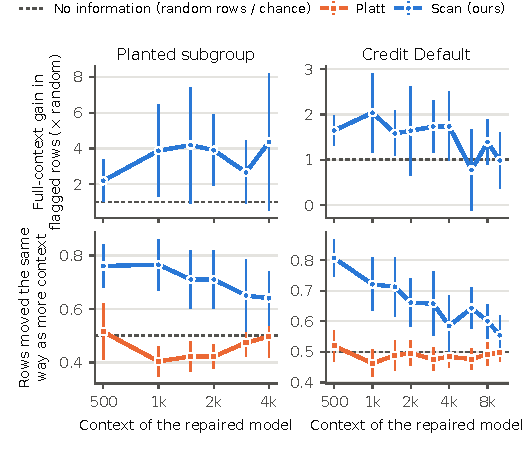
\includegraphics[width=\columnwidth]{fig_attribution.pdf}
\caption{Row-level attribution of the benefit from full TabPFN context (mean and 95\% CI over 10
seeds). Top: full-context improvement concentrated in rows flagged by Scan, divided by their share
of rows; $1\times$ is the random-row baseline. Bottom: fraction of corrected rows whose logit moves
in the same direction as the full-context model; 0.5 is chance. Platt is shown as a global-calibration
reference.}
\label{fig:attr}
\end{figure}

Similar aggregate log-loss does not by itself show that repair and additional context address the
same deficits. We therefore compare TabPFN at each context $k$ with the corresponding full-context
predictor row by row (Fig.~\ref{fig:attr}). Observations flagged by Structured Scan receive
\PlConcLo--\PlConcHi$\times$ their expected share of the improvement delivered by full context on
the planted problem, and \CrConcLo--\CrConcHi$\times$ on Credit for $k\le4$k; random rows would
receive $1\times$. At 500--1{,}000 context rows, Scan moves corrected logits in the same direction
as the full-context model in \PlSignLo--\PlSignHi\% of planted cases and
\CrSignLo--\CrSignHi\% of Credit cases. Platt's global transformation agrees in only
\PlattSignLo--\PlattSignHi\% of rows, approximately the chance baseline. This alignment weakens as
$k$ approaches full context and little incremental improvement remains. Thus, at constrained
contexts, Structured Scan preferentially identifies observations that later benefit from additional
context rather than merely producing a similar average loss.

\textbf{Resource accounting.} Repair and additional context use labelled data differently. A
repaired 1{,}000-row TabPFN uses held-out discovery and selection labels once to estimate its
post-hoc correction, whereas a larger frozen TabPFN places additional labelled rows directly in
context and pays for them on every subsequent prediction. The comparison below is therefore a
deployment-compute trade-off conditional on available labelled monitoring data, not a claim of equal
label consumption. All post-hoc corrections use the same discovery and selection resources. If all
held-out rows are instead placed into context (\PlLabCtx{} rows on the planted data, \CrLabCtx{} on
Credit), the frozen model is more accurate (test LL about \PlLabLL{} and \CrLabLL{}) but costs
\PlLabCpu$\times$ and \CrLabCpu$\times$ more CPU inference per prediction than the 1{,}000-row
model (\PlLabGpu$\times$ and \CrLabGpu$\times$ on the T4). Repair does not dominate context when
compute is free; its advantage is recurring compute when context is constrained by latency, memory
or a CPU budget.

\subsection{Repair versus context on the compute frontier}

\begin{figure*}[t]
\centering
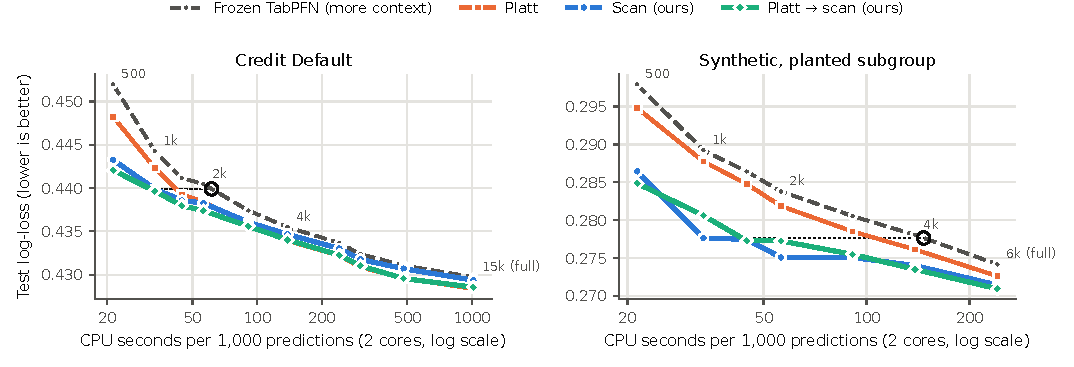
\includegraphics[width=\textwidth]{fig_frontier.pdf}
\caption{Test log-loss versus recurring TabPFN-2.5 prediction cost on a 2-core CPU; labels denote
context size. Post-hoc corrections are fitted once, so their one-time fit cost is excluded from the
horizontal axis and their recurring cost is essentially that of the underlying context. Dotted line
and open circle mark the frozen context whose loss matches Structured Scan applied at 1{,}000 rows.}
\label{fig:frontier}
\end{figure*}

\begin{table}[t]
\centering
\caption{Recurring context cost and equivalent-context accuracy. Top: seconds to score 1{,}000 rows at representative TabPFN-2.5 contexts. Bottom: for a correction fitted at 1{,}000 context rows, the frozen context needed to match its test loss and the corresponding recurring cost multiplier. Scan fitting is one-time (median 7.0\,s on one CPU core at a 1{,}000-row context).}
\label{tab:cost}
\footnotesize\setlength{\tabcolsep}{4pt}
\begin{tabular}{lrrrrr}
\toprule
Context & 500 & 1k & 2k & 4k & 15k \\
\midrule
CPU (s) & 21 & 33 & 56 & 139 & 1{,}017 \\
T4 GPU (s) & 1.0 & 1.4 & 2.3 & 5.1 & 38.9 \\
\bottomrule
\end{tabular}
\\[4pt]
\begin{tabular}{llrrr}
\toprule
Data & Fix at 1k & Equiv.\ context & CPU & T4 \\
\midrule
Planted & Platt & 1,238 & 1.2$\times$ & 1.2$\times$ \\
 & Scan & 4,175 & 4.4$\times$ & 3.8$\times$ \\
 & Platt$\to$scan & 2,973 & 2.7$\times$ & 2.4$\times$ \\
 & Boosted corrector & 3,411 & 3.3$\times$ & 2.9$\times$ \\
\midrule
Credit & Platt & 1,292 & 1.2$\times$ & 1.2$\times$ \\
 & Scan & 2,152 & 1.8$\times$ & 1.7$\times$ \\
 & Platt$\to$scan & 2,225 & 1.9$\times$ & 1.8$\times$ \\
 & Boosted corrector & 4,140 & 4.4$\times$ & 3.7$\times$ \\
\bottomrule
\end{tabular}
\end{table}


Because a fitted subgroup repair adds only a few rule comparisons at inference, its recurring cost
is essentially that of the underlying small-context TabPFN. Figure~\ref{fig:frontier} therefore
compares predictive loss with recurring prediction cost. At a 1{,}000-row context, Structured Scan
reaches a Credit test loss matched by the uncorrected model only at \CrEqScan{} context rows, and a
planted-subgroup loss matched at \PlEqScan{} rows. Achieving the same loss through additional
context makes each CPU prediction \CrEqScanCpu$\times$ and \PlEqScanCpu$\times$ more expensive,
respectively (\CrEqScanGpu$\times$ and \PlEqScanGpu$\times$ on the T4), whereas Scan requires a
one-time median CPU fit of \ScanSecOneMed\,s at this context. Platt buys only about
\PlEqPlattX--\CrEqPlattX$\times$ context. The boosted residual corrector buys more effective
context than Scan on Credit (\CrEqXgb{} rows versus \CrEqScan{}) but less on the planted structured
problem (\PlEqXgb{} versus \PlEqScan{}). These results define an operating regime rather than a
universal dominance claim: structured repair is attractive when additional context improves
accuracy but recurring context cost is the binding resource.

\subsection{Abstention as the model strengthens}
As confirmed localized residual structure disappears, a selective repair should intervene less. On
Credit, the fraction of seeds with an accepted Scan rule falls from \CrFiveInterv{} at 500 rows to
\CrFullInterv{} at full context, while the fraction of accepted rules passing the audit falls from
\CrFiveAudit{} to \CrFullAudit. In the no-planted-effect condition, mean Scan gain approaches zero
as context grows, although the nominal acceptance criterion still admits some spurious rules: from
2{,}000 rows onward, \NuHarmLo--\NuHarmHi{} of 10 seeds are made slightly worse, with a
nonsignificant mean change of $\NuFullScan$ at full context. In these foundation-model settings,
Platt$\to$scan has a positive mean at every context (\NuPSMin{} to \NuPSMax), consistent with
it first removing broad miscalibration before searching for localized residual structure. We therefore view
the two-stage variant as useful when global and local calibration errors coexist, rather than as a
universally superior form of Structured Scan.
%=====================================================================
\section{Exact CPU Acceleration of Structured Scan Repair}\label{sec:systems}
%=====================================================================
Profiling the reference implementation on the planted benchmark shows that approximately
\CostScorerShare\% of fit time is spent in the exact scorer~\eqref{eq:gain}, which is invoked
roughly 65{,}000 times for a standard 2{,}400-row, 30-feature discovery set. We therefore optimize
this bottleneck without changing the scanner's statistical decisions. First, a Numba
implementation~\cite{lam2015numba} fuses each Newton solve into one compiled loop while preserving
its iteration, clipping and stopping rules. Second, shortlisted thresholds for a
(feature, parent-rule) pair are scored in one compiled batch using lookup tables rather than
repeated set-membership operations. Third, independent candidates are evaluated in parallel while
retaining each candidate's original summation order.

These changes leave candidate scores, selected rules and fitted shifts unchanged in all
\SpConfigs{} synthetic configurations and on Credit Default. At the default problem size they
reduce one repair fit from \SpOrigDefault\,s to \SpBatDefault\,s, a \SpBatX$\times$ speed-up, and
give \SpBatMin--\SpBatMax$\times$ acceleration across the tested discovery sizes on a 2-core CPU
(Fig.~\ref{fig:cost}). Across the TabPFN context ladder, median fitting time is \ScanSecMed\,s on
one CPU core. Faster search also matters statistically: permutation-calibrated acceptance, a
principled way to control spurious selection after a large search, requires hundreds of repeated
scans.

\begin{figure}[t]
\centering
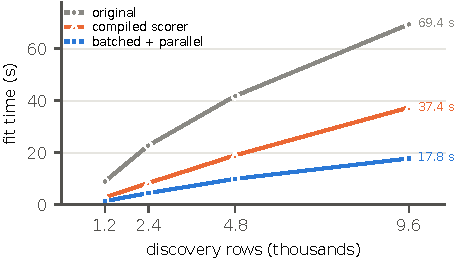
\includegraphics[width=0.94\columnwidth]{fig_cost.pdf}
\caption{Exact CPU acceleration of one Structured Scan fit as discovery size grows (30 features,
2-core CPU). The compiled scorer and the batched+parallel implementation preserve the reference
arithmetic and select identical rules; the latter gives 3.9--6.2$\times$ speed-up across the tested
sizes.}
\label{fig:cost}
\end{figure}

\textbf{Towards an accelerator kernel.} The acceleration above is exact. As a separate exploratory
direction, Eq.~\eqref{eq:gain} can be approximated for candidate screening by summarizing subgroup
logits into $B=64$ quantile bins, reducing each Newton solve to 64 aggregated values. On
\FidHistN{} random conjunctions this approximation selects the same best candidate and top 50 as
exact scoring, with maximum gain error \FidHistErr\,nats. With feature-wise prefix sums, threshold
screening becomes a dense (feature$\times$threshold$\times$bin) tensor operation suited to GPUs or
other accelerators; shortlisted candidates would still be re-scored exactly before selection.
%=====================================================================
\section{Discussion, Limitations and Outlook}
%=====================================================================
\textbf{What the results say.} In the controlled planted benchmark, strong predictors from two very
different tabular-learning paradigms all leave a comparable localized residual after base-model
construction. Global recalibration changes that defect only modestly, whereas Structured Scan can
remove most of it once sufficient discovery evidence is available. The 2{,}400$\to$9{,}600
experiment shows that failure to detect a known structured residual can be a sample-power problem
rather than a backbone-specific limitation. Credit shows the complementary regime: when a strong
in-distribution model leaves little validated localized residual, Scan mostly abstains, while global
recalibration or a higher-capacity residual learner may be more useful.

The correction methods therefore occupy distinct operating regimes rather than forming a single
ranking. Global calibration is appropriate when residual error is broad; a flexible boosted
residual learner can maximize predictive gain when additional correction complexity is acceptable;
Structured Scan is designed for sparse, interpretable localized errors that can be independently
validated and rejected when evidence is weak. For an in-context model this creates a second
trade-off: such a residual can be repaired once, or the base model can be strengthened by carrying
more context on every prediction.

\textbf{Limitations.} The empirical study uses one synthetic generator and one real dataset, and
the context--compute analysis is demonstrated only for TabPFN-2.5; broader validation across real
tabular tasks and other in-context models is needed. Structured subgroup discovery is data-hungry:
with 2{,}400 observations, a five-way conjunction among 30 features is frequently missed even when
the true residual remains substantial. The current acceptance rule also uses a nominal $p<0.05$
test after a large discovery search and can admit spurious rules when little structured signal
remains; permutation-calibrated acceptance is the natural next step.

The repair-versus-context comparison is a deployment-resource comparison, not an equal-label
comparison. If all available held-out labels are added directly to TabPFN's context and inference
compute is unconstrained, the larger-context model is more accurate. On Credit, the boosted residual
corrector also achieves greater raw log-loss improvement than Structured Scan. The value of Scan is
therefore its particular design point: a small number of named, validated subgroup corrections,
negligible incremental inference cost and explicit abstention. CPU timing uses the TabPFN-2.5
architecture with randomly initialized weights solely to measure architecture-level computation;
all predictive results use released model weights, and GPU timing uses those released weights on a
T4.

\textbf{Next steps.} The results motivate five extensions: (a) permutation-calibrated acceptance to
control search-induced false positives; (b) parallel per-feature screening and an accelerator-oriented
candidate-scoring kernel; (c) context-level repair, where examples from a detected subgroup are
added selectively to a foundation model's context rather than correcting its logits; (d) repair
under temporal shift (e.g. Bank Marketing~\cite{moro2014bank}) compared directly with refreshing
context using recent observations; and (e) structured correction inside model training, for example
a boosting procedure that can choose between a conventional tree update and an interpretable
subgroup shift. The last direction gives up the model-agnostic post-hoc property of the present
method and is therefore a distinct research problem.

\section*{Reproducibility}
Base-model logits are saved once for every dataset, seed and context, and all corrections, tables
and figures are regenerated from those frozen predictions on CPU. Canonical foundation-model runs
use a free-tier T4 GPU. Repeating TabICLv2 on an A100 changes frozen test log-loss by at most
$7\times10^{-5}$ per run; no accept/abstain decision changes, and only one of 30 fitted repairs
differs in rule count because a candidate lies at the acceptance threshold. The Credit Default
analysis uses the original UCI data and reproduces the earlier tree-model baseline (test LL
\CreditXGBbase{} versus 0.4341). Code released with the paper records the package versions, fixed
splits and random seeds used to regenerate all reported results.
\bibliographystyle{IEEEtran}
\bibliography{refs}

\end{document}
